% This file is generated by the MATLAB m-file laprint.m. It can be included
% into LaTeX documents using the packages graphicx, color and psfrag.
% It is accompanied by a postscript file. A sample LaTeX file is:
%    \documentclass{article}\usepackage{graphicx,color,psfrag}
%    \begin{document}% This file is generated by the MATLAB m-file laprint.m. It can be included
% into LaTeX documents using the packages graphicx, color and psfrag.
% It is accompanied by a postscript file. A sample LaTeX file is:
%    \documentclass{article}\usepackage{graphicx,color,psfrag}
%    \begin{document}% This file is generated by the MATLAB m-file laprint.m. It can be included
% into LaTeX documents using the packages graphicx, color and psfrag.
% It is accompanied by a postscript file. A sample LaTeX file is:
%    \documentclass{article}\usepackage{graphicx,color,psfrag}
%    \begin{document}% This file is generated by the MATLAB m-file laprint.m. It can be included
% into LaTeX documents using the packages graphicx, color and psfrag.
% It is accompanied by a postscript file. A sample LaTeX file is:
%    \documentclass{article}\usepackage{graphicx,color,psfrag}
%    \begin{document}\input{fig_N_vs_SNR_diff_pout_diff_maxContPow_th}\end{document}
% See http://www.mathworks.de/matlabcentral/fileexchange/loadFile.do?objectId=4638
% for recent versions of laprint.m.
%
% created by:           LaPrint version 3.16 (13.9.2004)
% created on:           06-Jan-2016 16:54:20
% eps bounding box:     16 cm x 12 cm
% comment:              
%
%\begin{psfrags}%
%\psfragscanon%
%
% text strings:
\psfrag{s03}[b][b]{\fontsize{8.5}{12.75}\fontseries{m}\mathversion{normal}\fontshape{n}\selectfont \color[rgb]{0,0,0}\setlength{\tabcolsep}{0pt}\begin{tabular}{c}$\tau$ [ms]\end{tabular}}%
\psfrag{s04}[t][t]{\fontsize{8.5}{12.75}\fontseries{m}\mathversion{normal}\fontshape{n}\selectfont \color[rgb]{0,0,0}\setlength{\tabcolsep}{0pt}\begin{tabular}{c}$\gamma$ [dB]\end{tabular}}%
%
% axes font properties:
\fontsize{8.5}{12.75}\fontseries{m}\mathversion{normal}%
\fontshape{n}\selectfont%
%
% xticklabels:
\psfrag{x01}[t][t]{-20}%
\psfrag{x02}[t][t]{-15}%
\psfrag{x03}[t][t]{-10}%
\psfrag{x04}[t][t]{-5}%
%
% yticklabels:
\psfrag{v01}[r][r]{0}%
\psfrag{v02}[r][r]{2}%
\psfrag{v03}[r][r]{4}%
\psfrag{v04}[r][r]{6}%
\psfrag{v05}[r][r]{8}%
\psfrag{v06}[r][r]{10}%
\psfrag{v07}[r][r]{12}%
\psfrag{v08}[r][r]{14}%
\psfrag{v09}[r][r]{16}%
\psfrag{v10}[r][r]{18}%
\psfrag{v11}[r][r]{20}%
%
% Figure:
%\resizebox{8cm}{!}{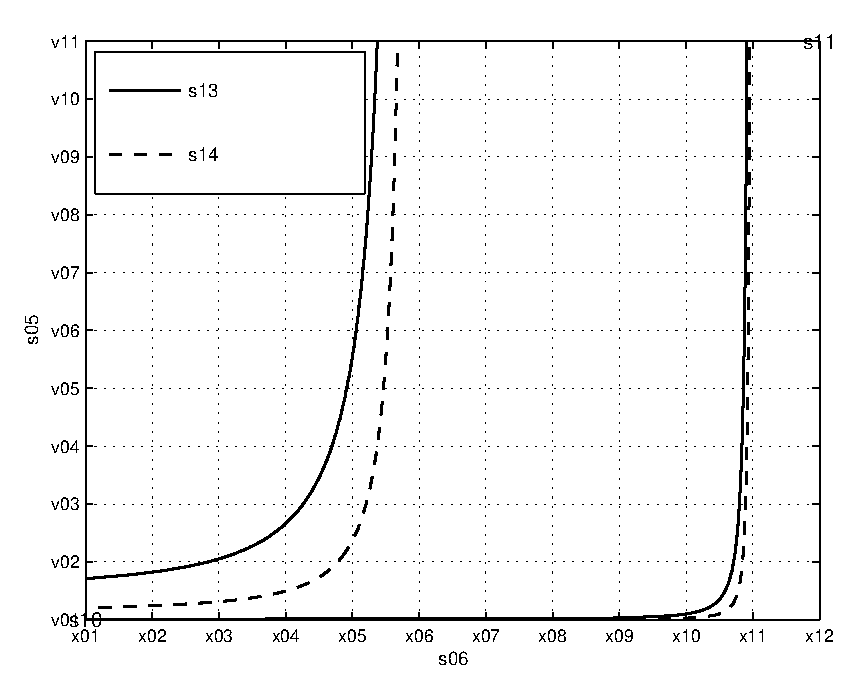
\includegraphics{fig_N_vs_SNR_diff_pout_diff_maxContPow_th.eps}}%
%\end{psfrags}%
%
% End fig_N_vs_SNR_diff_pout_diff_maxContPow_th.tex
\end{document}
% See http://www.mathworks.de/matlabcentral/fileexchange/loadFile.do?objectId=4638
% for recent versions of laprint.m.
%
% created by:           LaPrint version 3.16 (13.9.2004)
% created on:           06-Jan-2016 16:54:20
% eps bounding box:     16 cm x 12 cm
% comment:              
%
%\begin{psfrags}%
%\psfragscanon%
%
% text strings:
\psfrag{s03}[b][b]{\fontsize{8.5}{12.75}\fontseries{m}\mathversion{normal}\fontshape{n}\selectfont \color[rgb]{0,0,0}\setlength{\tabcolsep}{0pt}\begin{tabular}{c}$\tau$ [ms]\end{tabular}}%
\psfrag{s04}[t][t]{\fontsize{8.5}{12.75}\fontseries{m}\mathversion{normal}\fontshape{n}\selectfont \color[rgb]{0,0,0}\setlength{\tabcolsep}{0pt}\begin{tabular}{c}$\gamma$ [dB]\end{tabular}}%
%
% axes font properties:
\fontsize{8.5}{12.75}\fontseries{m}\mathversion{normal}%
\fontshape{n}\selectfont%
%
% xticklabels:
\psfrag{x01}[t][t]{-20}%
\psfrag{x02}[t][t]{-15}%
\psfrag{x03}[t][t]{-10}%
\psfrag{x04}[t][t]{-5}%
%
% yticklabels:
\psfrag{v01}[r][r]{0}%
\psfrag{v02}[r][r]{2}%
\psfrag{v03}[r][r]{4}%
\psfrag{v04}[r][r]{6}%
\psfrag{v05}[r][r]{8}%
\psfrag{v06}[r][r]{10}%
\psfrag{v07}[r][r]{12}%
\psfrag{v08}[r][r]{14}%
\psfrag{v09}[r][r]{16}%
\psfrag{v10}[r][r]{18}%
\psfrag{v11}[r][r]{20}%
%
% Figure:
%\resizebox{8cm}{!}{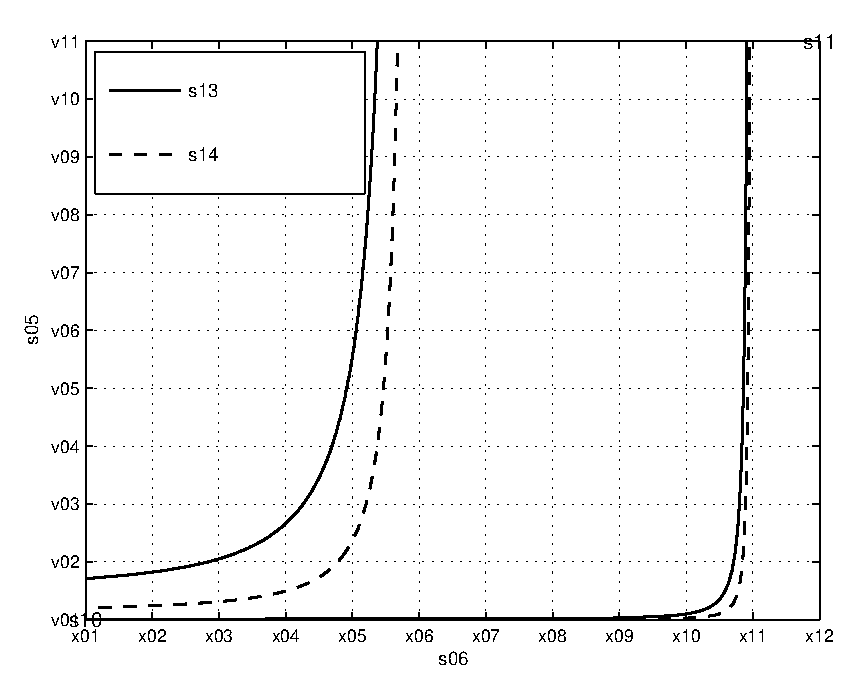
\includegraphics{fig_N_vs_SNR_diff_pout_diff_maxContPow_th.eps}}%
%\end{psfrags}%
%
% End fig_N_vs_SNR_diff_pout_diff_maxContPow_th.tex
\end{document}
% See http://www.mathworks.de/matlabcentral/fileexchange/loadFile.do?objectId=4638
% for recent versions of laprint.m.
%
% created by:           LaPrint version 3.16 (13.9.2004)
% created on:           06-Jan-2016 16:54:20
% eps bounding box:     16 cm x 12 cm
% comment:              
%
%\begin{psfrags}%
%\psfragscanon%
%
% text strings:
\psfrag{s03}[b][b]{\fontsize{8.5}{12.75}\fontseries{m}\mathversion{normal}\fontshape{n}\selectfont \color[rgb]{0,0,0}\setlength{\tabcolsep}{0pt}\begin{tabular}{c}$\tau$ [ms]\end{tabular}}%
\psfrag{s04}[t][t]{\fontsize{8.5}{12.75}\fontseries{m}\mathversion{normal}\fontshape{n}\selectfont \color[rgb]{0,0,0}\setlength{\tabcolsep}{0pt}\begin{tabular}{c}$\gamma$ [dB]\end{tabular}}%
%
% axes font properties:
\fontsize{8.5}{12.75}\fontseries{m}\mathversion{normal}%
\fontshape{n}\selectfont%
%
% xticklabels:
\psfrag{x01}[t][t]{-20}%
\psfrag{x02}[t][t]{-15}%
\psfrag{x03}[t][t]{-10}%
\psfrag{x04}[t][t]{-5}%
%
% yticklabels:
\psfrag{v01}[r][r]{0}%
\psfrag{v02}[r][r]{2}%
\psfrag{v03}[r][r]{4}%
\psfrag{v04}[r][r]{6}%
\psfrag{v05}[r][r]{8}%
\psfrag{v06}[r][r]{10}%
\psfrag{v07}[r][r]{12}%
\psfrag{v08}[r][r]{14}%
\psfrag{v09}[r][r]{16}%
\psfrag{v10}[r][r]{18}%
\psfrag{v11}[r][r]{20}%
%
% Figure:
%\resizebox{8cm}{!}{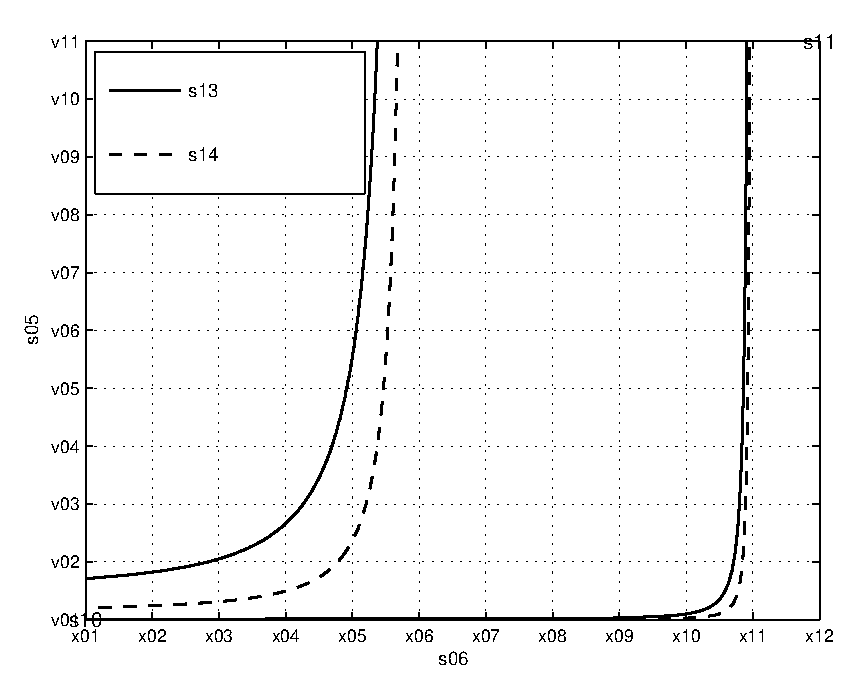
\includegraphics{fig_N_vs_SNR_diff_pout_diff_maxContPow_th.eps}}%
%\end{psfrags}%
%
% End fig_N_vs_SNR_diff_pout_diff_maxContPow_th.tex
\end{document}
% See http://www.mathworks.de/matlabcentral/fileexchange/loadFile.do?objectId=4638
% for recent versions of laprint.m.
%
% created by:           LaPrint version 3.16 (13.9.2004)
% created on:           31-Aug-2015 16:25:39
% eps bounding box:     16 cm x 12 cm
% comment:              
%
%\begin{psfrags}%
%\psfragscanon%
%
% text strings:
\psfrag{s05}[b][b]{\fontsize{8.5}{12.75}\fontseries{m}\mathversion{normal}\fontshape{n}\selectfont \color[rgb]{0,0,0}\setlength{\tabcolsep}{0pt}\begin{tabular}{c}$\tau$ [ms]\end{tabular}}%
\psfrag{s06}[t][t]{\fontsize{8.5}{12.75}\fontseries{m}\mathversion{normal}\fontshape{n}\selectfont \color[rgb]{0,0,0}\setlength{\tabcolsep}{0pt}\begin{tabular}{c}$\gamma$ [dB]\end{tabular}}%
\psfrag{s10}[][]{\fontsize{10}{15}\fontseries{m}\mathversion{normal}\fontshape{n}\selectfont \color[rgb]{0,0,0}\setlength{\tabcolsep}{0pt}\begin{tabular}{c} \end{tabular}}%
\psfrag{s11}[][]{\fontsize{10}{15}\fontseries{m}\mathversion{normal}\fontshape{n}\selectfont \color[rgb]{0,0,0}\setlength{\tabcolsep}{0pt}\begin{tabular}{c} \end{tabular}}%
\psfrag{s12}[l][l]{\fontsize{8.5}{12.75}\fontseries{m}\mathversion{normal}\fontshape{n}\selectfont \color[rgb]{0,0,0}$\opc = 0.1$}%
\psfrag{s13}[l][l]{\fontsize{8.5}{12.75}\fontseries{m}\mathversion{normal}\fontshape{n}\selectfont \color[rgb]{0,0,0}$\opc = 0.01$}%
\psfrag{s14}[l][l]{\fontsize{8.5}{12.75}\fontseries{m}\mathversion{normal}\fontshape{n}\selectfont \color[rgb]{0,0,0}$\opc = 0.1$}%
%
% axes font properties:
\fontsize{8.5}{12.75}\fontseries{m}\mathversion{normal}%
\fontshape{n}\selectfont%
%
% xticklabels:
\psfrag{x01}[t][t]{-20}%
\psfrag{x02}[t][t]{-18}%
\psfrag{x03}[t][t]{-16}%
\psfrag{x04}[t][t]{-14}%
\psfrag{x05}[t][t]{-12}%
\psfrag{x06}[t][t]{-10}%
\psfrag{x07}[t][t]{-8}%
\psfrag{x08}[t][t]{-6}%
\psfrag{x09}[t][t]{-4}%
\psfrag{x10}[t][t]{-2}%
\psfrag{x11}[t][t]{0}%
\psfrag{x12}[t][t]{2}%
%
% yticklabels:
\psfrag{v01}[r][r]{0}%
\psfrag{v02}[r][r]{2}%
\psfrag{v03}[r][r]{4}%
\psfrag{v04}[r][r]{6}%
\psfrag{v05}[r][r]{8}%
\psfrag{v06}[r][r]{10}%
\psfrag{v07}[r][r]{12}%
\psfrag{v08}[r][r]{14}%
\psfrag{v09}[r][r]{16}%
\psfrag{v10}[r][r]{18}%
\psfrag{v11}[r][r]{20}%
%
% Figure:
%\resizebox{8cm}{!}{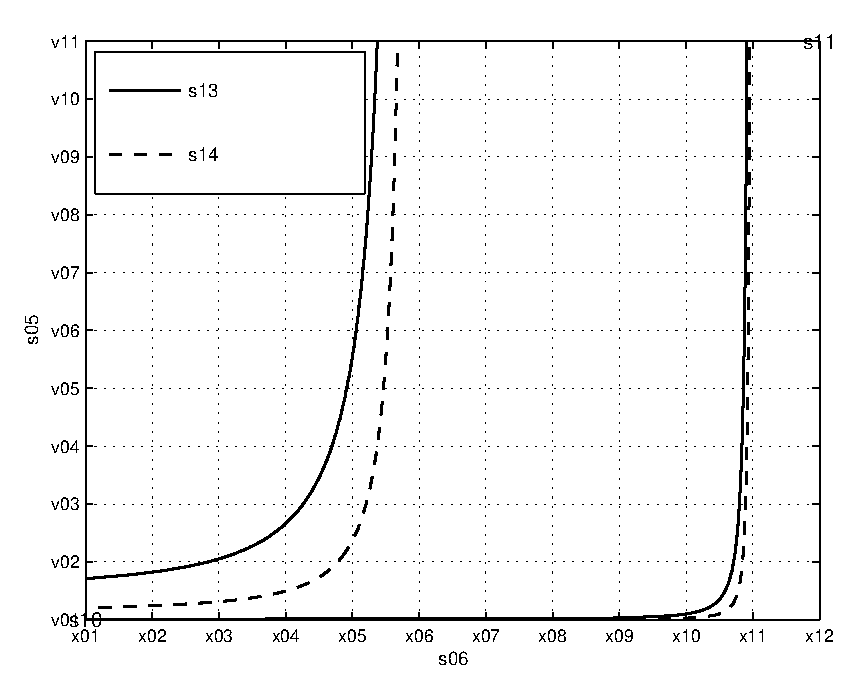
\includegraphics{fig_N_vs_SNR_diff_pout_diff_maxContPow_th.eps}}%
%\end{psfrags}%
%
% End fig_N_vs_SNR_diff_pout_diff_maxContPow_th.tex
